\documentclass{beamer}

\usepackage{graphicx}
\usepackage{fontspec}

\usetheme{Berlin}

\setmainfont{Times New Roman}

\title{Neurosymbolic Methods for Dynamic Knowledge Graphs}
\subtitle{Research Methodologies and Academic Writing}
\author{Uif\u{a}lean Paul-Adrian}
\institute{Babe\c{s}-Bolyai University}
\date{November 18, 2024}

\begin{document}
    \begin{frame}
        \titlepage
    \end{frame}

    \begin{frame}{Outline}
        \tableofcontents
    \end{frame}

    \begin{frame}{Research Goal}
        \begin{itemize}
            \item Formalize the representation of Dynamic Knowledge Graphs (DKGs)
            \item Focus on:
            \begin{itemize}
                \item Dynamic Knowledge Graph Completion (KG Completion)
                \item Dynamic Entity Alignment
            \end{itemize}
            \item Neurosymbolic methods for temporal \& non-temporal DKGs
            \item Address challenges of current approaches
        \end{itemize}
    \end{frame}

    
    \section{Introduction to Knowledge Graphs}
    
    \begin{frame}{What is a Knowledge Graph?}
        \begin{itemize}
            \item Knowledge Graphs (KGs) organize information in a structured format with entities and relationships.
        \end{itemize}
        
        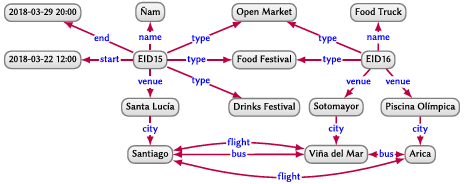
\includegraphics[width=\textwidth]{KG.png}
    \end{frame}

    \begin{frame}{Overview of Evolving Knowledge Graphs}
        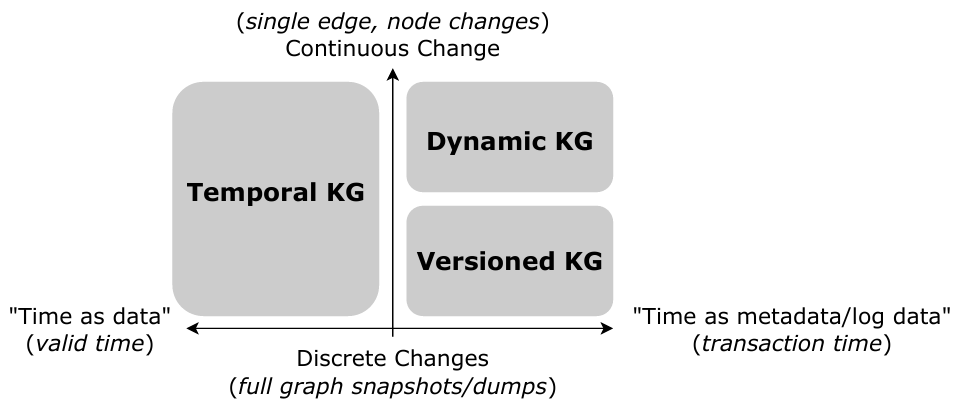
\includegraphics[width=\textwidth]{evolving-KGs.png}
    \end{frame}

    \begin{frame}{Static and Temporal Knowledge Graphs}
        Static Knowledge Graph (KG):
        \begin{itemize}
            \item A directed labeled graph: \( G = (E, R, L, F) \)
            \item \( E \): entities, \( R \): relations, \( L \): literals, \( F \): facts
            \item Example: \{Barack Obama, USA\}, relation: \{president of\}, fact: \{(Barack Obama, president of, USA)\}
        \end{itemize}
        Temporal Knowledge Graph (TKG):
        \begin{itemize}
            \item Includes time intervals: \( G = (E, R, L, T, Q) \)
            \item \( Q \): quadruples with time intervals: \{(Barack Obama, president of, USA, [2009, 2017])\}
        \end{itemize}
    \end{frame}

    \begin{frame}{Dynamic Knowledge Graphs}
        Dynamic Knowledge Graph (DKG):
        \begin{itemize}
            \item Sequence of KGs indexed by time steps: \( \{G_{t0}, G_{t1}, \dots, G_{tn}\} \)
            \item Transition between snapshots based on additions/removals of entities, relations, literals, and facts.
        \end{itemize}
        Example of Dynamic Update:
        \begin{itemize}
            \item \( G_0 \): \{Barack Obama, USA\}, fact: \{(Barack Obama, president of, USA)\}
            \item \( G_1 \): \{Donald Trump, USA\}, fact: \{(Donald Trump, president of, USA)\}
            \item Temporal extension: \( G_0 \) updated with \{(Donald Trump, president of, USA, [2017, 2021])\}
        \end{itemize}
    \end{frame}
    
    \begin{frame}{Techniques to Represent Temporal Information in KGs - (1)}
        \begin{itemize}
            \item XML Schema Properties: \texttt{xsd:dateTime}, \texttt{xsd:duration}, \texttt{xsd:date}, etc.
            \item Temporal Properties: Time-specific attributes in relationships.
            \item Example: \texttt{:Alice :employmentStart "2020-01-01"^^xsd:date}
            
            \item Reification: Attach metadata (e.g. time) to triples.
            \item Example: \texttt{_:statement :since "2022-01-01"^^xsd:date}
            
            \item Time Ontology (OWL): Models temporal concepts: instants, intervals, durations.
            \item Example: \texttt{ex:JobStart a time:Instant ; time:inXSDDateTime "2020-01-01T00:00:00Z"^^xsd:dateTime}
            \item Reasoning: Define classes like \texttt{LongTermEmployee} based on temporal conditions (e.g., works since before "2021-01-01").
        \end{itemize}
    \end{frame}

    \begin{frame}{Techniques to Represent Temporal Information in KGs - (2)}
        \begin{itemize}
            \item Named Graphs: Group triples with metadata (e.g., temporal context).
            \item Example: \texttt{GRAPH <http://example.org/graph/2022-01-01> \{ :Alice :knows :Bob . \}}
            \item Quadruples: Extend RDF triples with a fourth element (context or timestamp).
            \item Example: \texttt{:Alice :knows :Bob "2022-01-01"^^xsd:date .}
            
            \item RDF-star: Compact representation for complex facts.
            \item Example: \texttt{<< :Alice :knows :Bob >> :since "2022-01-01"^^xsd:date}
            
            \item Versioning: Track historical changes in KGs.
            \item Example: \texttt{:Document123 :hasVersion :Version1 . :Version1 :timestamp "2024-01-01T10:00:00Z" .}
        \end{itemize}
    \end{frame}
    
    \begin{frame}{Prominent Knowledge Graphs}
        \begin{itemize}
            \item DBpedia:
            \begin{itemize}
                \item Temporal properties: \texttt{dbo:birthDate}, \texttt{dbo:deathDate}.
                \item Versioning: DBpedia Live, historical snapshots.
            \end{itemize}
            \item YAGO:
            \begin{itemize}
                \item Temporal relations: \texttt{wasBornOnDate}, \texttt{happenedOnDate}.
                \item RDF-star for detailed annotations.
            \end{itemize}
            \item Wikidata:
            \begin{itemize}
                \item Qualifiers for temporal context: start/end dates.
                \item Full edit history for dynamic updates.
            \end{itemize}
            \item EventKG:
            \begin{itemize}
                \item Event modeling: \texttt{sem:hasBeginTimeStamp}, \texttt{sem:hasEndTimeStamp}.
                \item Extends Simple Event Model for temporal relations.
            \end{itemize}
        \end{itemize}
    \end{frame}
     

    \section{Dynamic KG Completion}

    \begin{frame}{Neurosymbolic Methods}
        \begin{itemize}
            \item Combines symbolic reasoning with neural networks.
            \item Key components: 
            \begin{itemize}
                \item Symbolic: Logic, rules, ontologies.
                \item Neural: Data learning, generalization.
        \end{itemize}
        \item Applications: 
        \begin{itemize}
            \item KG completion, temporal reasoning, hybrid models.
        \end{itemize}
        \item Benefits: 
        \begin{itemize}
            \item Improved interpretability, scalability, integration.
        \end{itemize}
        \end{itemize}
    \end{frame}

    \begin{frame}{Dynamic Knowledge Graph Completion}
        \begin{itemize}
            \item Goal: Predict missing links and adapt to evolving information.
            \item Methods are divided into:
                \begin{itemize}
                    \item Interpolation-based: Predicts missing data using existing knowledge
                    \item Extrapolation-based: Forecasts future relations based on past knowledge snapshots.
                \end{itemize}
        \end{itemize}
        \begin{figure}[h!]
            \centering
            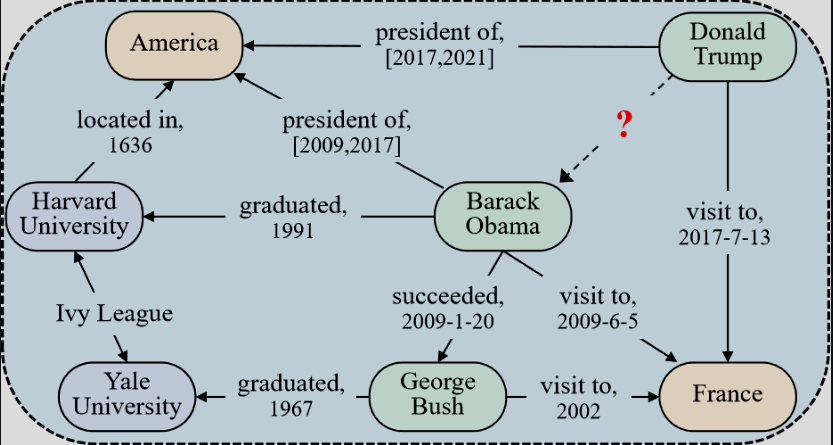
\includegraphics[width=0.45\textwidth]{interpolation.png}
            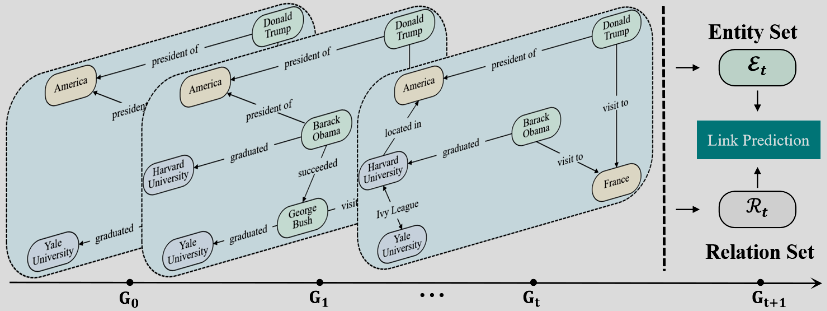
\includegraphics[width=0.45\textwidth]{extrapolation.png}
        \end{figure}
    \end{frame}

    \begin{frame}{Temporal Knowledge Graph Completion (TKGC)}
        \begin{itemize}
            \item Evolving over time, often incomplete or biased.
            \item Link Prediction with temporal context:
            \begin{itemize}
                \item Predict missing tail, head, or relation in a fact.
            \end{itemize}
            \item Methods focus on:
            \begin{itemize}
                \item Embeddings sensitive to timestamps
                \item Temporal functions for better modeling
                \item Deep learning for sequence and structural patterns
            \end{itemize}
            \item Training:
            \begin{itemize}
                \item Negative sampling generates incorrect quadruplets.
                \item Loss functions optimize for prediction accuracy.
            \end{itemize}
            \item Evaluation Metrics: Mean Rank, Mean Reciprocal Rank (MRR)
        \end{itemize}
    \end{frame}

    \begin{frame}{Dynamic Knowledge Graphs (DKGs)}
        \begin{itemize}
            \item DKGs evolve over time; re-training is costly.
            \item Online learning challenges:
            \begin{itemize}
                \item Prone to catastrophic forgetting
            \end{itemize}
            \item Solution: Continual Learning (CL) to update embeddings incrementally.
        \end{itemize}
    \end{frame}

    \begin{frame}{Continual KG Embedding and Methods}
        \begin{itemize}
            \item Continual KG Embedding:
            \begin{itemize}
                \item Fine-tuning reduces re-training.
                \item Low-rank adapters (IncLoRA): Modular updates for efficiency.
            \end{itemize}
            \item Methods:
            \begin{itemize}
                \item puTransE: Multi-embedding for dynamic relations.
                \item DKGE: Embedding with GCN and attention.
                \item LKGE: Context via masked subgraphs.
                \item IncLoRA: Efficient updates for dynamic graphs.
            \end{itemize}
        \end{itemize}
    \end{frame}

    
    \section{Dynamic Entity Alignment}
    
    \begin{frame}{Dynamic Entity Alignment}
        \begin{itemize}
            \item Align entities between two KGs over time
            \item Handles evolving data during alignment
            \item Combines structural, temporal, and attribute information
        \end{itemize}
    \end{frame}

    \begin{frame}{Temporal EA Methods}
        \begin{itemize}
            \item Methods use GCNs/GNNs with temporal attention
            \item Key approaches:
            \begin{itemize}
                \item Time-aware GCN: Uses reverse links and attention for relation weighting
                \item Tem-EA: Combines RNNs and embeddings for similarity across KGs
                \item Temporal Matching: Simple matching mechanism, avoids complex embeddings
                \item Adaptive Graph Networks: Employs graph attention for temporal aggregation
                \item DualMatch: Encodes relational and temporal information for alignment
            \end{itemize}
        \end{itemize}
    \end{frame}

    \begin{frame}{Temporal and Evolving EA Methods}
        \begin{itemize}
           \item Temporal Relational Entity Alignment (TREA):
            \begin{itemize}
                \item Maps entities, relations, timestamps into a unified space
                \item Uses GNN with temporal relational attention for feature integration
                \item Includes time regularization for handling unseen timestamps
            \end{itemize}
            \item Incremental Temporal Entity Alignment (ITEA):
            \begin{itemize}
                \item Combines GAT (teacher) and GCN (student) with knowledge distillation
                \item Multi-head GNN for time-aware structural embeddings
                \item Aligns new entities using similarity measures like string matching
            \end{itemize}
        \end{itemize}
    \end{frame}

    \begin{frame}{ITEA: Training and Knowledge Distillation}
        \begin{itemize}
            \item Knowledge Distillation:
            \begin{itemize}
                \item Teacher model (GAT): Learns complex temporal/structural features
                \item Student model (GCN): Efficient training with sampled nodes
            \end{itemize}
            \item Loss combines standard classification with distillation for alignment
            \item Incremental training allows new entity embeddings without retraining the entire model
        \end{itemize}
    \end{frame}

    
    \section{Conclusions}
    
    \begin{frame}{Conclusion}
        \begin{itemize}
            \item Explored DKG types, KG representation, and alignment methods.
            \item Challenges:
            \begin{itemize}
                \item Overlooks schematic or ontological information.
                \item Limited adaptability to real-world, large-scale KGs.
                \item Underutilization of literal information in KGs.
            \end{itemize}
            \begin{columns}
            \begin{column}{0.5\textwidth}
                \begin{itemize}
                    \item Large Language Models (LLMs):
                    \begin{itemize}
                        \item Few-shot learning for TKGC showed limited performance gains.
                        \item Lack of analysis on hallucinations or overgenerations.
                    \end{itemize}
                \end{itemize}
            \end{column}
            \begin{column}{0.5\textwidth}
                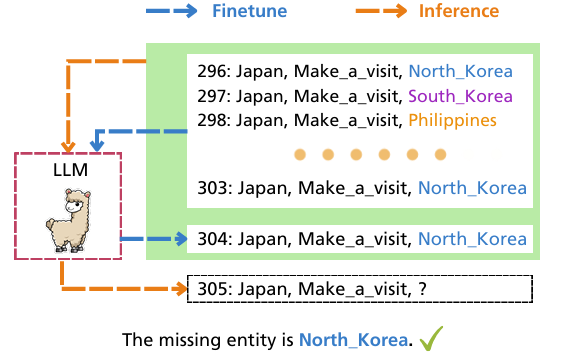
\includegraphics[width=\linewidth]{LLM.png}
            \end{column}
        \end{columns}
        \end{itemize}
    \end{frame}

    \begin{frame}{Personal Proposal}
        
    \end{frame}

    \begin{frame}{References}
    \footnotesize
        \begin{thebibliography}{99}

        \bibitem{Hogan2022}
        Hogan A, Blomqvist E, Cochez M, d’Amato C, de Melo G, Gutierrez C, et al. Knowledge Graphs. \textit{ACM Computing Surveys}. 2022;54(4):71:1-71:37. Available from: \url{https://doi.org/10.1145/3447772}.
        
        \bibitem{Polleres2023}
        Polleres A, Pernisch R, Bonifati A, Dell’Aglio D, Dobriy D, Dumbrava S, et al. How Does Knowledge Evolve in Open Knowledge Graphs? \textit{TGDK}. 2023;1(1):11:1-11:59.

        \bibitem{Wang2023}
        Wang J, Wang B, Qiu M, Pan S, Xiong B, Liu H, et al. A survey on temporal knowledge graph completion: Taxonomy, progress, and prospects. \textit{arXiv preprint arXiv:230802457}. 2023.

        \bibitem{Luo2024}
        Luo R, Gu T, Li H, Li J, Lin Z, Li J, et al. Chain of History: Learning and Forecasting with LLMs for Temporal Knowledge Graph Completion. \textit{CoRR}. 2024;abs/2401.06072. Available from: \url{https://doi.org/10.48550/arXiv.2401.06072}.

    \end{thebibliography}
    \end{frame}
\end{document}